The Schr\"{o}dinger operator for a vanishing potential if given by
\bse 
\Hf := -\frac{\hbar^2}{2m} \Laplace
\ese 
and it corresponds to the energy observable for a free particle\footnote{Free particle here means what we think of classically as a free particle, it experiences no potential.} of mass $m$. 

This lecture aims to derive the spectrum of $\Hf$ and use it to study the time evolution of pure states. We shall consider $d=3$ throughout this lecture, and shall make use of the results of last lecture heavily. We shall also use units such that $m=\frac{1}{2}\hbar^2$ in order to lighten notation; i.e. $\Hf=-\Laplace$.

\subsection{Domain of Self Adjointness of $\Hf$}

If we want to talk about $\Hf$ being an observable, we need to show that it is self adjoint on some domain. From (i) in \Cref{prop:FourierDerivatives} it follows that 
\bse 
\fF(-\Laplace\psi)(p) = |p|^2 (\fF\psi)(p) =: (P^2\widehat{\psi})(p),
\ese 
where $|p|^2 := p_1^2+p_2^2+p_3^2$. In other words, 
\bse 
\fF(-\Laplace \psi) =: P^2\widehat{\psi}.
\ese 

\br 
The physicists says "in momentum space the Laplacian acts simply by multiplication of the norm of the momentum, $|p|^2$".
\er 

We can now rewrite the above by inserting $\id_{L^2(\R^3)}=\fF^{-1}\fF$ to give 
\bse 
\fF \circ \Hf \circ \fF^{-1}\circ \fF\psi = P^2 \circ \fF\psi ,
\ese 
from which is follows
\bse 
\fF\Hf\fF^{-1} = P^2,
\ese 
whose maximal domain is 
\bse 
\cD_{P^2} = \{\widehat{\psi}\in L^2(\R^3) \, | \, P^2 \widehat{\psi} \in L^2(\R^3) \}.
\ese 

\bt 
A maximally defined real multiplication operator is self adjoint on its maximal domain. 
\et 

\bq 
Let
\bi{rrCl}
A : & \cD_A & \to & \cH \\
& \psi & \mapsto & a\psi 
\ei 
where $a\in\R$ and $\cD$ is the maximal domain of $A$ (i.e. there are no elements outside this domain such that $a\psi\in\cH$). This operator is clearly symmetric as, for $\psi,\varphi\in\cD$
\bi{rCl}
\braket{\psi}{A\varphi} & = & \braket{\psi}{a\varphi} \\
& = & a\braket{\psi}{\varphi} \\
& = & \braket{\overline{a}\psi}{\varphi} \\
& = & \braket{a\psi}{\varphi} \\
& = & \braket{A\psi}{\varphi}.
\ei 
We have therefore $A\se A^*$, which means $\cD_A\se \cD_{A^*}$ with $A^*\psi=A\psi$ for all $\psi\in\cD_A$, but $\cD_A$ is maximal so there is no $\psi\notin \cD_A$ such that $A^*\psi=a\psi\in\cH$ and so $\cD_{A^*}\se \cD_A$. Therefore $A=A^*$ on this maximal domain.
\eq 

From this theorem, then, we have that $\fF\Hf\fF^{-1}$ is self adjoint on the domain $\cD_{P^2}$. 

\subsection{Spectrum of $\Hf$}

One can quickly find the spectrum of $\Hf$ using the resolvent map, 
\bse
R_{P^2} (z) = \frac{1}{|p|^2-z},
\ese 
from which is clearly follows that the resolvent set is simply 
\bse 
\rho(P^2) = \{z\in\C \, | \, z \neq |p|^2 \}. 
\ese 
Then using the fact that $|p|^2\in\R$ with $|p|^2 >0$\footnote{We use a strict equality as if $|p|^2 =0$ then there is no momentum and so the operator $P^2$ just maps it to 0.} we have 
\bse 
\rho(P^2) = \C\setminus\R^+_0.
\ese 
Then finally using the definition of the spectrum as the compliment of the resolvent set we get 
\bse 
\sigma(\Hf) = \sigma(P^2) = \R^+_0.
\ese 

\br 
This is not the method used in the lectures, which I\footnote{I being Richie} find more confusing. As I don't fully understand the latter parts of the proof provided (I think the main idea is introducing a form of the spectral theorem in which the integral is performed over the spectrum of the operator and then use the characteristic function Dr. Schuller introduced) I shall not type it up here to avoid potential confusion to the readers. If you do follow the complete method please feel free to contact me and I can add it and give you credit. 
\er 

\bp 
For every self adjoint operator there is always some transformation which transforms the operator into a mere multiplication operator.
\ep 

\br 
Once you know the transformation the self adjoint operator of interest, the spectrum always follows by the same method. 
\er 

\subsection{Time Evolution}

Recall that Axiom 4 tells us the evolution of a state is given by\footnote{We're using units such that $\hbar=1$.} 
\bse 
\rho_{\psi_{t_2}} = e^{-i(t_2-t_1)H} \rho_{\psi_{t_1}} e^{i(t-2-t_1)H},
\ese 
which for a pure state becomes 
\bse 
\frac{\braket{\psi_{t_2}}{\cdot}}{\braket{\psi_{t_2}}{\psi_{t_2}}}\psi_{t_2} = e^{-i(t_2-t_1)H} \frac{\braket{\psi_{t_1}}{\cdot}}{\braket{\psi_{t_1}}{\psi_{t_1}}}\psi_{t_1} e^{i(t_2-t_1)H}.
\ese 
If we now choose to view the RHS as the following composition 
\bse 
\frac{1}{\braket{\psi_{t_1}}{\psi_{t_2}}} \Big(e^{-i(t_2-t_1)H}\braket{\psi_{t_1}}{\cdot}\Big) \circ \Big( \psi_{t_1} e^{i(t_2-t_1)H}\Big) \textcolor{blue}{ = \frac{1}{\braket{\psi_{t_1}}{\psi_{t_2}}} \Big(e^{-i(t_2-t_1)H}\ket{\psi_{t_1}}\Big)\circ\Big(\bra{\psi_{t_1}}e^{i(t_2-t_1)H}\Big) },
\ese 
it follows that we can represent the time evolution of a pure \emph{state} via the evolution of the \emph{Hilbert space element} as
\bse  
\psi_{t_2} = e^{-i(t_2-t_1)H}\psi_{t_1}.
\ese  

\br 
We are assuming here that $H$ is time-independent. If it wasn't you would simply use an integral in the exponential.
\er 

\br 
We should note that in the above time is viewed as a parameter, not a coordinate --- i.e. this is \emph{not} a spacetime picture. The elements $\psi_{t_1}$ and $\psi_{t_2}$ are simply elements of the Hilbert space, each of which is associated to a different time. This can be compared to saying classically that the position of a particle is an element of $\R^3$, and at a later time its position is still an element of $\R^3$, although potentially a different one. 
\er 

Now for the free particle we have 
\bse 
\fF^{-1} P^2 \fF = \Hf,
\ese 
which, along with the fact that $P^2$ is a multiplicative operator, gives us 
\bse 
e^{-it\Hf} \fF^{-1} = \fF^{-1}e^{-itP^2}.
\ese 
Acting both sides on $\widehat{\psi}:= \fF\psi$ gives 
\bse 
e^{-it\Hf}\psi = \fF^{-1}\Big( p \mapsto e^{-it|p|^2} \cdot \widehat{\psi}(p) \Big),
\ese 
which a convolution of functions. It is then tempting to use use 
\bse 
f*g = (2\pi)^{d/2}\fF^{-1}\big((\fF f)\cdot (\fF g)\big)
\ese 
to give us\footnote{Remember $d=3$ here.} 
\bi{rCl}
e^{-it\Hf}\psi(x) = \frac{1}{(2\pi)^{3/2}} \Big(\fF^{-1}\big(p\mapsto e^{-it|p|^2}\big) * \psi\Big)(x),
\ei 
and then use \Cref{lem:FourierExponentialSquare} to give
\bse 
\fF^{-1}\big(p\mapsto e^{-it|p|^2}\big)(x) = \frac{1}{(2t)^{3/2}} e^{-\frac{1}{4it}|x|^2},
\ese 
however there is a problem with both of these steps. 

Firstly for us to use the convolution theorem we require both functions to be $L^1(\R^3)$. For $\psi$ we can simply take the intersection $\psi\in L^2(\R^3)\cap L^1(\R^3)$, however the exponential term is unavoidably not in $L^1(\R^3)$ (if you take the absolute value you get 1, and then integrating over all of $\R^3$ gives a divergent result). On top of that, in order to use \Cref{lem:FourierExponentialSquare} we require the real part of the coefficient to be strictly positive (in order to avoid the branch cut), but $\Re(it)=0$. 

Luckily we can fix both of these problems with the same step, regularisation. We regularise both by introducing a positive, real factor into the exponential and then taking the limit, 
\bse 
e^{-it|p|^2} = \lim_{\varepsilon\to0} e^{-(it+\varepsilon)|p|^2}.
\ese 
The addition of $\varepsilon$ stops the integral diverging (because of the minus sign) and we also have $\Re(it+\varepsilon) = \varepsilon >0$ and so we can use \Cref{lem:FourierExponentialSquare}.

So, using the continuity of the product and the inverse Fourier transform we have 
\bi{rCl}
e^{-it\Hf}\psi(x) & = & \bigg[\lim_{\varepsilon\to0} \bigg( x\mapsto \frac{1}{(2\pi)^{3/2}} \frac{1}{\big(2(it+\varepsilon)\big)^{3/2}} \exp\Big( -\frac{|x|^2}{4(it+\varepsilon)}\Big) \bigg)* \psi\bigg](x) \\
& := & \lim_{\varepsilon\to0} \frac{1}{\big(4\pi(it+\varepsilon)\big)^{3/2}} \int_{\R^3}d^3y \exp\bigg( -\frac{|x-y|^2}{4(it+\varepsilon)}\bigg) \psi(y).
\ei 
Finally using dominated convergence to take the limit inside the integral, we have\footnote{Note $t=t_2-t_1$ here.}
\bse 
\psi_{t_2}(x) = \frac{1}{(i4\pi t)^{3/2}} \int_{\R^3}d^3y \exp\bigg( - \frac{|x-y|^2}{i4t}\bigg) \psi_{t_1}(y).
\ese 

\subsection{Physical Interpretation (for the Patient Observer)}

After massaging the above result a bit we arrive at the famous `\emph{spreading of the wavefunction}' result.

First start by expanding 
\bse 
|x-y|^2 = |x|^2 + |y|^2 - 2xy
\ese 
to give 
\bse 
\psi_{t_2}(x) = \frac{\exp\Big( - \frac{|x|^2}{i4t}\Big)}{(i4\pi t)^{3/2}} \int_{\R^3} d^3y \exp\bigg( -i\frac{x}{2t} y\bigg) \exp\bigg( - \frac{|y|^2}{i4t}\bigg) \psi_{t_1}(y),
\ese 
which is a Fourier transform with result 
\bse 
\psi_{t_2}(x) = \frac{\exp\Big( - \frac{|x|^2}{i4t}\Big)}{(i2t)^{3/2}} \cdot \reallywidehat{\exp\Big( - \frac{|y|^2}{i4t}\Big) \psi_{t_1}(y)} \bigg(\frac{x}{2t}\bigg).
\ese 

We now use the fact that we have a patient observer (i.e. one who watches for a long time) to take the asymptotic behaviour\footnote{That is take the limit $t\to\infty$ at places where it wont cause problems.} to give 
\bse 
\psi_{t_2}(x) \sim \frac{\exp\Big( - \frac{|x|^2}{i4t}\Big)}{(i2t)^{3/2}} \widehat{\psi}_{t_1}\bigg(\frac{x}{2t}\bigg),
\ese 
which, if the $\psi$s were viewed as `waves' (i.e. plots on a graph) would indicate that the `wave spreads out over time'. In other words, simplifying to $\R$ instead of $\R^3$ we'd have something along the following diagram.
\begin{center}
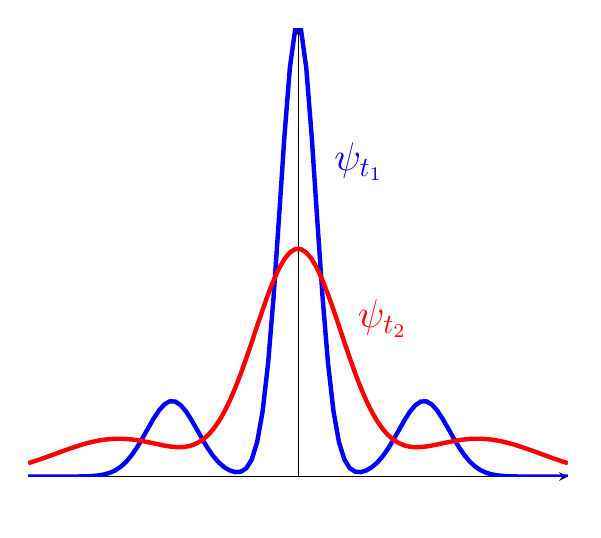
\begin{tikzpicture}
\begin{axis}[ticks=none,axis lines=middle]
    \addplot [domain=-15:15, samples=100, ultra thick, blue] {6*exp((-x*x)/2) + exp((-(x+7)^2)/4) +  exp((-(x-7)^2)/4)};
    \addplot [domain=-15:15, samples=100, ultra thick, red] {3*exp((-x*x)/12) + 0.5*exp((-(x+10)^2)/24) +  0.5*exp((-(x-10)^2)/24)};
\end{axis}
\node at (4.2,4) {\textcolor{blue}{\Large{$\psi_{t_1}$}}};
\node at (4.5,2) {\textcolor{red}{\Large{$\psi_{t_2}$}}};
\node at (6.8,-0.3) {\Large{$\R$}};
\end{tikzpicture}
\end{center}
So the function appears to spread out (keeping the area under it constant) over time. 